%%%%%%%%%%%%
\documentclass[11pt]{article}
\usepackage{latexsym}
\usepackage{amsmath}
\usepackage{graphicx}
\usepackage{amssymb}
\DeclareGraphicsExtensions{.pdf,.png,.jpg}
\usepackage[top=1in, bottom=1in, left=1in, right=1in]{geometry}
\usepackage{pgfplots}
\pgfplotsset{width=7cm,compat=1.8}
\parindent0pt
\usepgfplotslibrary{statistics}
\parskip\bigskipamount

\begin{document}

\centerline{\textbf{2018 INFORMS O.R. {\&} Analytics Student Team Competition -- ENTRY FORM}}

\baselineskip16pt plus 1pt minus 1pt


\textbf{Entry Number: [}2018ORASTC252]

\textbf{Executive Summary (not to exceed 2 pages)}\\*


\textbf{Team Makeup {\&} Process}\\*

\textbf{Framing the Problem}\\*
%Rebalancing을 위한 로직 (turnover 반영)
%파라메터 $\gamma$ 반영방법?!
%Robustness


\textbf{Data}\\*
\begin{itemize}
\item[1.] The Structure of the Data %데이터 구조 및 분석
\item[] The data from Principal consists of 3 parts which are timeseries data, riskmodels data, and result template data. 
\begin{itemize}
	\item Time Series Data :
	\begin{itemize}
		\item[] 
	\end{itemize}
	\item Riskmodels Data :
	\begin{itemize}
		\item[] 
	\end{itemize}
	\item Result Template Data :
	\begin{itemize}
		\item[] 
	\end{itemize}
\end{itemize}

\item[2.] Data Pre-processing and Rescailing

	% 왜 data preprocessing이 필요한가. 어떤 방식으로 하였는가 (전반적)
	\item[ ] There are some difficulties in applying the data given from Principal directly to the model. Therefore, we present the following data preprocessing process. To make the data composed of three parts more flexible, a process of data preprocessing formed dataframe using the Pandas Library(http://pandas.pydata.org) in Python. 
	
	% Timeseries를 가지고 있는 Time Series Data 및 Result Template Data를 날짜별로 추출
	In particular, as rebalancing is carried out, it is configured to extract not all time series data, but only the data needed for the iteration. The parameters used in model were extracted from data frames formed for each period, when each parameter (Alpha Score($\alpha$), Beta($\beta$),4 Weekly Returns ($r$), etc) was set with the 'SEDOL' index as the key value. This dictionary data type is proper to consider a list of assets that may change every period.
	
	% Riskmodel Data에서 Omega(Risk Matrix)를 추출하는 방식
	The parameter Omega ($ \Omega $) is specified as the covariance matrix for a given data. In this case, the index in the columns and rows are 'SEDOL', the key value of the time series dictionary derived from the above, and are constructed in the form of full matrix. 
	
	% Quadratic 을 표현하기 위해 필요한 정제 (????)
	
	%Data Rescailing
	%\omega * \omega 와 alpha score(범위 : -2.08e-05~1.93e-05) 의 값이 너무 작음 --> Python의 한계수치로 인한 계산 오류 발생 가능성 및  Optimization Tool CPLEX에서 값이 무시되는 경우 가 생길 수 있음.
	
\item[3.] The Analysis of the Data
	% MCAPQ 와 SECTOR별 Weight의 범위 (결과?와 연관지어서)
	% Active Share과 Tracking Error의 관계 (데이터 기반)
	% 추가 historical 데이터 확보 및 분석 --> omega 도출 결과 corelation이 낮음 => 이유 간단히 분석?
	
\end{itemize}

\textbf{Methodology Approach {\&} Model Building}\\*
\begin{itemize}

\item[\textbf{1.}] \textbf{Formulation Approach}
	\item[] \underline{\textbf{Model Building}}:
	% CPLEX를 가지고 QCQP 풀었을 경우 (1) Linearlize (2) Handling non-convex constraints -> Bisearch Approach (3)간단한 실험 (4)실험결과 분석 (문제를 어렵게 만드는 제약조건 , cardinality 제약식)
	Before buiding the model, we tried to solve the  Quadratic Constraint Quadratic Programming (QCQP)  problem by using the IBM CPLEX, which is well known Optmization tool, to determine the difficulty of the problem. Since CPLEX can not deal with non-linear constraints,the given formulation is required to be reformulated. 
	First, the constraints (9) are reformulated as follows:
	\begin{align*}
	\text{(9*)} \quad
	& y_i \geq w_i, \quad \forall i \in N \\
	& y_i \leq w_i + 0.999 \quad \forall i \in N \\
	& 50 \leq \sum_{i \in N} y_i \leq 70 \\
	& y_i \in \{0,1\}, \quad \forall i \in N 
	\end{align*}
	The decision variables $y_i$ is 1 if asset $i \in N$ is selected where $w_i$ is bigger than 0. Because $w_i \leq 0.001$ is considered to $w_i = 0$,  $y_i = 0$ if $w_i = 0$. The opposite is the same as well. Constraints (10) and (11) are also non-linear. However, if non-convex constraints are linearized, they significantly impact speed by increasing the number of variables to determine and the number of constraints to consider. In other words, it is very inefficient to reformulate constraints (10) and (11), which represent the limits of Active Share and Tracking Error, respectively. Therefore, after solving the problem without reflecting constraints (10) and (11), we tried to identify the following observations.
	\begin{itemize}
		\item[] \textbf{Observation1.} In most cases, the range of Active Share is satisfied.
		\item[] \textbf{Observation2.} Tracking Error is less than lower bound (0.05).
		%\item[] \textbf{Observation3.} The portfolio weights($w$) tend to be less than the benchmark weights($w_{\text{bench}}$).
	\end{itemize}
	According to observation2, Tracking Error should be raised. At this time, $d^T\Omega d$ can be expressed as $\quad w^T\Omega  w - w_{\text{bench}}^T\Omega  w_{\text{bench}} \quad$, which means that the difference between the benchmark weight and the portfolio weight is too small that TE does not satisfy the lower bound.In other words, the difference between the two weights must be increased to some extent to satisfy the constraints. Since the following $  w_{\text{bench}}^T\Omega  w_{\text{bench}}  $ is fixed, it is required to satisfy the constraints by changing $w^T\Omega  w $. 
	Because the weight value of all of the unselected assets from approximately 500 candidates is zero, the weight value is equal to or less than the benchmark weight value. On the other hand, the weight value of the 50 to 70 selected assets may be larger or smaller than the benchmark weights. If the portfolio weight is further increased in the case of the portfolio weight is bigger than benchmark weight, the difference between the two weights will be positively increased. In the opposite case, portfolio weight is less than benchmark weight, the difference between to two weights(Active Weight) will be negatively increased by reducing portfolio weight.
	\item[] \underline{\textbf{Bisectional Algorithm}}:
	 We applied the idea to the bisectional search algorithm.  The bisectional search algorithm is an iterative algorithm that narrows the range and finds a feasible solution. When narrowing the range, if the feasible solution exists in the range, search in the right range based on the median of the range, and search in the left range if the feasible solution does not exist.
	
	An example is shown in \ref{fig:bisection}. Let  $ \sum_{p\in P} w_p = 0.6$, where $P$ is a set of assets whose $d$ is greater than zero. First, the solution is searched by dividing the interval between 0.6 and 1.0. If the solution is a feasible solution that satisfies both the range of Active Share and Tracking Error, narrow the range and search again in the left section.  The search is stopped when the width of the range($\underline{Z} \sim \overline{Z}$) is less than the end condition which is set to 0.001. 
	
	\begin{figure}[h] 
		\begin{center}
			\includegraphics[width=0.75\textwidth]{bisection}
			\caption{An Example of Bisectional Search} \label{fig:bisection}
		\end{center}
	\end{figure}

	%$\sum_{p \in P} w_i = (\underline{Z} +\overline{Z})/2 $
	% bisectional algorithm 결론
	
	%\item[]\underline{Evolutionary Approach} : 
	
	% 진화 알고리즘 (ex.EDA)으로 접근. (간단한 실험?) -> 문제점 도출 : population의 수를 크게 두고 여러번 풀어 확률적 이론 등을 적용시키는 데에는 오랜시간 소요.
		
	\item[\textbf{2.}] \textbf{Neural Network Approach}

	\item[]\underline{\textbf{The application of GAN}} : \textbf{Generative adversarial networks (GANs)} are well known deep neural net(NN) architectures comprised of two networks. One neural network, called the  \textbf{Generator(G)}, generates new data instances, while the other, the  \textbf{Discriminator(D)}, decides whether each instance of data is real dataset or not. Both neural networks learn to alternate with each other. The G trains to generate data similar to real data, and the D trains to distinguish real data from fake data generated by G. 

		\begin{figure}[h] 
		\begin{center}
			\includegraphics[width=0.6\textwidth]{GAN_basic}
			\caption{The strucutre of basic GAN} \label{fig:GAN-basic}
		\end{center}
	\end{figure}

See \ref{fig:GAN-basic}. G generates fake data when arbitrary noise z is given as a input through a NN composed of layers which are a input layer, multiple hidden layers and a output layer. G tries to make $D(x) = 1$ for sample x extracted from fake data, and D tries to make $D(G (z)) = 0$ for sample $G (z)$ , where $z \sim p_{z}(z)$. Therefore, the loss function $V(D,G)$ of GAN can be expressed as follows : %reference?
 \begin{align*}
 \min_G \max_D V(D,G)  = \mathbb{E}_{x~p_{data}(x)}[\log D(x)]  + \mathbb{E}_{x~p_{x}(x)}[\log(1-D(G(z)))] 
 \end{align*}
 We use the GAN 's basic idea of learning networks with adversarial relationships between two networks to solve the problem of portfolio optimization. G determines the decision variable $w$ of the formulation, and D determines if the data generated from G is feasible. D is based on the formulation, and the sample data $G(z)$ generated in G checks both the feasibility of the solution and the quality of objective value. Therefore, the value of loss in D is the sum of the degree of violation from the constraints and objective value. G is a deep NN structure consisting of one input layer, three hidden layers and one ouput layer. G tries to minimize the loss of D for the sample $G(z)$ generated from the random input noise $z \sim \mathcal {U}(-1,1)$. That is, the decision variable $ w $ generated in G is trained to be feasible for all constraints and the objective value to be minimized. Unlike the basic GAN structure, GAN for portfolio optimization has G for NN structure, but D is not, and only G is required to train. The loss function $V(G)$ of GAN can be expressed as follows :
 \begin{align*}
 \min_G \mathbb{E}_{x~p_{data}(x)}[\log(D(G(z)))] 
 \end{align*}
%내용 추가 및 간단한 실험

\begin{figure}[h] 
	\begin{center}
		\includegraphics[width=0.6\textwidth]{GAN_port}
		\caption{The strucutre of GAN for portfolio optimization} \label{fig:GAN-port}
	\end{center}

\end{figure}
	
\item[\textbf{3.}] \textbf{GAN-MP Hybrid Approach} %이름 
	\item[] We propose a new \textbf{GAN(Generative adversarial networks)-MP(Mathmatical Programming) Hybrid approach} that complements the disadvantages of formluation approach and neural network approach and enhances their advantages.Several limitations could be derived from the three approaches we present above. When solving the problem with the formulation appraoch, we could not find a reasonable solution because to consider about 500 assets per iteration the number of decision variables to decide and the number of constraints to be satisfied are too high . Especially, constraints (9) which select cardinalities considering the target range on number of stocks make the problem difficult. 
	In the case of Neural Network Approach, there is a great advantage in that a solution that does not get significantly out from the whole constraints and that has a good objective value can be considered at the same time. However, it is difficult to find a soluton satisfying the feasibility for all the constraints and the fact that the training time takes too much time. The GAN-MP hybrid approach is a highly efficient approach that maximizes the advantages of GAN and formulation-based optimizations. This appraoch consists of three steps as shown in Figure 4. Step1 is the process of finding the cardinality set which is the combination of the selected assets. The cardinality set selected in Step1 solves the QCQP problem with the selected assets fixed and finds the local optimal solution. According to the result of Step2, the update algorithm finds cardinality set that can reduce the objective value and improves the solution.
	\begin{figure}[h] 
		\begin{center}
			\includegraphics[width=0.45\textwidth]{flowchart}
			\caption{A Flowchart of Hybrid Approach} \label{fig:flowchart}
		\end{center}
	\end{figure}

	\item[]\underline{\textbf{Step1. Initial Cardinality Set}}  :
	 When the number of assets to be considered is large, the problem becomes large as the number of constraints increases as well as decision variables. Thus, step1 filters out good assets that are crucial for minimizing the objective value. The combination of assets is chosen to minimize the risk and maximize return. In order to do this, the whole assets are required to consider. We propose a formulation approach that finds the solution through Mixed Integer Programming (MIP) and a neural network-based GAN as a way to satisfy constraints and to take low values of objective value globally. The following experiments were conducted to evaluate the performance of the algorithms.
	 \begin{itemize}
	 	\item Experiment Environment
	 	\begin{itemize}
	 		\item Number of Experiments : 50 times
	 		\item Experiement Time of MIP and GAN : 60 seconds
	 		\item Solver of MIP : Cplex
	 		\item Deep Learning Library : Pytorch
	 		\item The range of assets selected : 60 $\sim$ 70  
	 	\end{itemize}
 	
 		\item Experiment Results :
	 \end{itemize}
	 \begin{figure}[h]
	 \begin{center}
	 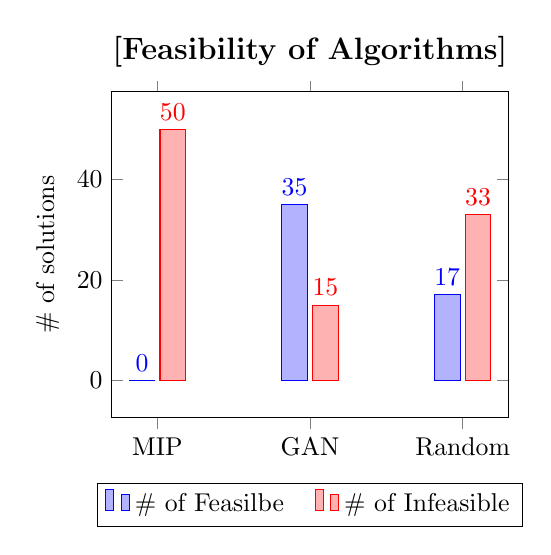
\begin{tikzpicture}[scale=0.93]
	 \begin{axis}[
	 ybar,
	 enlargelimits=0.15,
	 legend style={at={(0.5,-0.20)},
	 	anchor=north,legend columns=-1},
	 ylabel={\# of solutions},
	 symbolic x coords={MIP,GAN, Random},
	 xtick=data,
	 nodes near coords,
	 nodes near coords align={vertical},
	 	title={\large\textbf{[Feasibility of Algorithms]}}
	 ]
	 \addplot coordinates {(MIP,0) (GAN,35) (Random,17)};
	 \addplot coordinates {(MIP,50) (GAN,15) (Random,33)};
	 \legend{\# of Feasilbe$\quad$, \# of Infeasible}
	 \end{axis}
	 \end{tikzpicture} 
	 	\quad
	 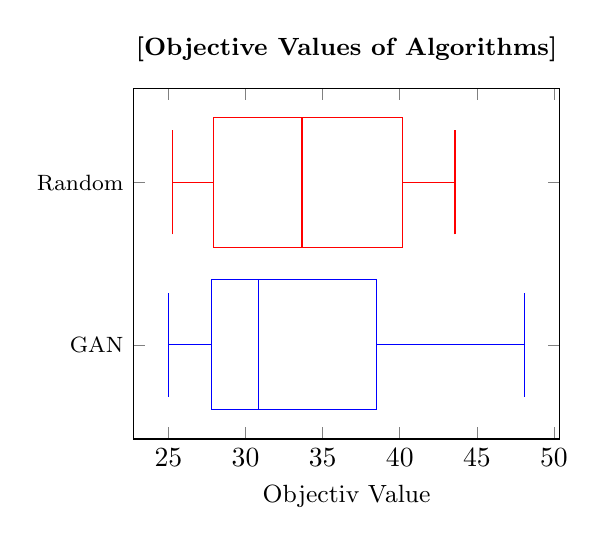
\begin{tikzpicture}[scale=1.]
	 \begin{axis}
	 [
	 ytick={1,2},
	 yticklabels={\footnotesize GAN, \footnotesize Random},
	 xlabel={\small Objectiv Value  },
	 	title={\small\textbf{[Objective Values of Algorithms]}}
	 ]
	 \addplot+[
	 boxplot prepared={
	 	median=30.83,
	 	upper quartile=38.47,
	 	lower quartile=27.77,
	 	upper whisker=48.08,
	 	lower whisker=25.02
	 },
	 ] coordinates {};
	 \addplot+[
	 boxplot prepared={
	 	median=33.65625795734167,
	 	upper quartile=40.18,
	 	lower quartile=27.90,
	 	upper whisker=43.58,
	 	lower whisker=25.25
	 },
	 ] coordinates {};
	 
	 \end{axis}
	 \end{tikzpicture}
	 
	 			\caption{Result of Algorithms} \label{fig:feasi}
	 	 \end{center}
 	 	\end{figure}
	  

\begin{figure}[h] 
	\begin{center}
		\includegraphics[width=0.6\textwidth]{step1}
		\caption{A Flowchart of Hybrid Approach} \label{fig:step1}
	\end{center}
\end{figure}


	


\end{itemize}
\textbf{Analytics Solution and Results}\\*




\begin{itemize}
\item \underline {This Entry Form}: Present your solution and results in this section, including completion of the Portfolio Performance Statistics chart below. You may supplement your analysis with additional charts, diagrams and/or other visualization; these supplements must be incorporated into this section of the Entry From.
\end{itemize}

\begin{center}
\textbf{Portfolio Performance Statistics}\vspace*{-14pt}
\end{center}
\begin{table}[htbp]
\def\arraystretch{1.4}
\begin{center}
\begin{tabular}{|l|c|c|}
\hline
\textbf{2007-01-01 to 2016-12-31}& 
\textbf{Portfolio}& 
\textbf{Benchmark} \\
\hline
Cumulative Return& 
{\%}& 
{\%} \\
\hline
Annualized Return& 
{\%}& 
{\%} \\
\hline
Annualized Excess Return& 
{\%}& 
-- \\
\hline
Annualized Tracking Error& 
{\%}& 
-- \\
\hline
Sharpe Ratio& 
& 
 \\
\hline
Information Ratio& 
& 
-- \\
\hline
\end{tabular}
\label{tab1}
\end{center}
\end{table}

\begin{itemize}
\item \underline {Results Template}: Populate and submit your numerical results using the Results Template. This template is provided as a separate file on the Competition download site. You can use either the Excel or CSV version.
\end{itemize}

\textbf{References}

\bgroup
\parskip0pt

Please follow guidelines in the \textit{Chicago Manual of Style,} 16$^{\text{th}}$ Edition. Here are examples: 

\begin{itemize}
\item[--] Journal article: Flynn J, Gartska SK (1990) A dynamic inventory model with periodic auditing. \textit{Oper. Res.} 38(6):1089--1103. 
\item[--] Book: Makridakis S, Wheelwright SC, McGee VE (1983) \textit{Forecasting: Methods and Applications}, 2nd ed. (John Wiley {\&} Sons, New York). 
\item[--] Edited Book: Martello S, Toth P (1979) The 0-1 knapsack problem. Christofides N, Mingozzi A, Sandi C, eds. \textit{Combinatorial Optimization} (John Wiley {\&} Sons, New York), 237--279.
\item[--] Online reference, fictional example: American Mathematical Institute (2005) Better predictors of geospatial variability. Retrieved June 14, 2005, \underline {www.mathematicsinstitute}.

\end{itemize}

\egroup

\end{document}
